
\section{Contenidos}

En esta sección se desarrollan contenidos relacionados a la gestión de almacenamiento masivo. Incluyendo conceptos y tecnologías. Los temas comprendidos serán: 

\begin{enumerate}
	\item   Arquitectura de E/S, Dispositivos de E/S (particionado), Filesystems (sistemas de archivos). 
	\item	Software RAID (implementación Linux MD), instalación y mantenimiento, niveles 0, 1, 10, 5.
	\item	Manejadores de volúmenes lógicos (implementación de LVM), instalación y mantenimiento
	\item	Diseños típicos de almacenamiento
\end{enumerate}


\section{Dispositivos y sistemas de archivos (filesystems)}

\subsection{Dispositivos lógicos}
Los \textbf{dispositivos lógicos de bloques} están asociados a algún medio de almacenamiento, real o virtual.  Ejemplos de dispositivos de bloques que encontramos con frecuencia son \lstinline$/dev/sda, /dev/sda1, /dev/dvd$, etc. Estos estarán asociados a algún medio, como puede ser un disco  magnético, una memoria de estado sólido o un archivo dentro de un sistema de archivos, por mencionar algunas posibilidades. En general se encontrarán bajo el directorio \lstinline$/dev$ dentro de la FSH (Filesystem Hierarchy).


Los dispositivos lógicos presentan una interfaz que provee direccionamiento random o directo, es decir, sus bloques están numerados y se puede acceder a cualquier bloque con independencia de cuál haya sido accedido anteriormente (operación de \emph{seek}). Pueden directamente contener un sistema de archivos u ofrecer soporte a otros dispositivos virtuales, que los agrupan (como los dispositivos RAID) o en general los utilizan (como los dispositivos snapshot de LVM). Los dispositivos de bloques más usuales con los que nos encontramos son los discos y las particiones, pero es interesante conocer otros dispositivos que están soportados por volúmenes lógicos, archivos, u otros, remotos, que se acceden por medio de la red. 

Desde el punto de vista del administrador/ora de sistemas, los archivos de dispositivo serán el medio para interactuar y gestionar el espacio provisto por el medio virtual o físico que representan. Es así que, por ejemplo, a través de una herramienta como fdisk, podemos dar una estructura al espacio en un disco magnético a través de la creación de una tabla de particiones sobre el dispositivo lógico asociado, por ejemplo: \lstinline$fdisk /dev/sda$ 

\begin{figure}[H]
\begin{center}
        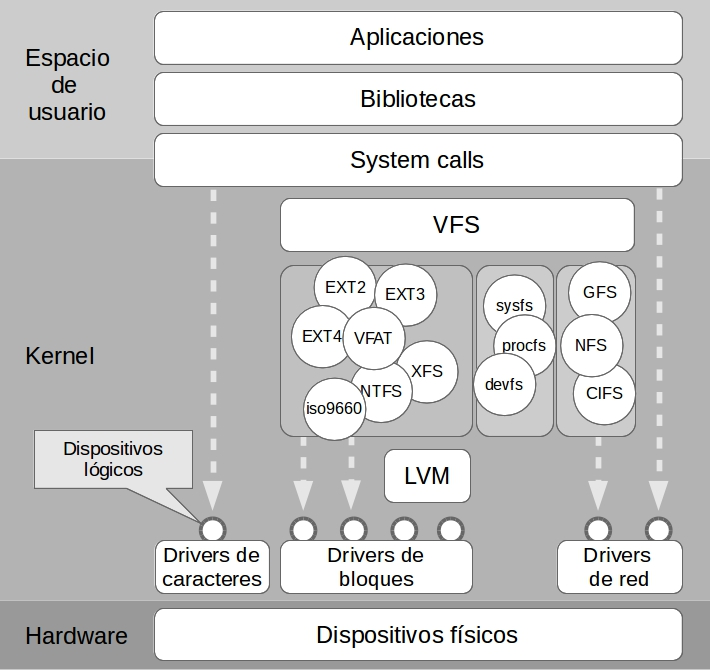
\includegraphics[scale=0.5, angle=0.0]{img/IO.jpg}
        \caption{Esquema IO y dispositivos}
        \label{module}
\end{center}
%\figura[14]{IO}{I/O y dispositivos}{IO.jpg} 
\end{figure}
\subsection{Dispositivos de bucle (loop devices)}

Los dispositivos de bucle (\lstinline$/dev/loop*$) de los 
sistemas GNU/Linux nos permiten \textbf{asociar} 
un archivo de dispositivo (bajo el directorio \lstinline$/dev$) con un 
\textbf{archivo
regular} dentro de un sistema de archivos. Esta funcionalidad nos permite, por 
ejemplo, montar un sistema de archivos que se encuentre contenido dentro del 
archivo regular (como puede ser una imagen ISO), o realizar pruebas simulando
la presencia de múltiples dispositivos. 

Dentro de esta asignatura se desarrollarán tecnologías que permiten la 
combinación de distintos medios de almacenamiento, con diferentes fines, 
por lo que utilizaremos los dispositivos de bucle para simular una 
infraestructura con múltiples discos físicos. 

La siguiente secuencia muestra la forma en que utilizaremos los dispositivos
de bucle con un ejemplo.

\begin{lstlisting}
Creando archivos regulares: 
$ dd if=/dev/zero of=imagen.img bs=1024 count=1024
1024+0 records in
1024+0 records out
1048576 bytes (1.0 MB) copied, 0.00223564 s, 469 MB/s
$ ls -l imagen.img
-rw-r--r-- 1 root root 1048576 Sep  1 11:54 imagen.img

Asociando dispositivos loop a archivos regulares: 
$ losetup /dev/loop0 imagen.img
$ losetup -a
/dev/loop0: [0808]:2260385 (/tmp/imagen.img)

Creando sistema de archivos en el dispositivo asociado: 
$ mkfs -t ext3 /dev/loop0
mke2fs 1.42.8 (20-Jun-2013)

Filesystem too small for a journal
Discarding device blocks:          done                            
Filesystem label=
OS type: Linux
Block size=1024 (log=0)
Fragment size=1024 (log=0)
Stride=0 blocks, Stripe width=0 blocks
128 inodes, 1024 blocks
51 blocks (4.98%) reserved for the super user
First data block=1
Maximum filesystem blocks=1048576
1 block group
8192 blocks per group, 8192 fragments per group
128 inodes per group

Allocating group tables: 0/1	done                            
Writing inode tables: 0/1	done                            
Writing superblocks and filesystem accounting information: 0/1	done

Montando el sistema de archivos para su uso: 
$ mkdir mnt
$ mount -o loop /dev/loop0 mnt
$ df -h mnt
Filesystem      Size  Used Avail Use% Mounted on
/dev/loop0     1003K   17K  915K   2% /tmp/mnt
$ ls -l mnt
total 12
drwx------ 2 root root 12288 Sep  1 11:54 lost+found

Utilizando el sistema de archivos: 
$ ls / > mnt/lista.txt
$ ls -l mnt
total 13
-rw-r--r-- 1 root root   167 Sep  1 11:54 lista.txt
drwx------ 2 root root 12288 Sep  1 11:54 lost+found
$ df -h mnt
Filesystem      Size  Used Avail Use% Mounted on
/dev/loop0     1003K   18K  914K   2% /tmp/mnt

Redimension del archivo regular de base, aumento: 
$ dd if=/dev/zero of=imagen.img bs=1024 count=1024 oflag=append conv=notrunc
1024+0 records in
1024+0 records out
1048576 bytes (1.0 MB) copied, 0.00206669 s, 507 MB/s
$ ls -l imagen.img
-rw-r--r-- 1 root root 2097152 Sep  1 11:54 imagen.img

Indicando al mecanismo de bucle el cambio en el archivo regular: 
$ losetup -c /dev/loop0
$ losetup -a
/dev/loop0: [0808]:2260385 (/tmp/imagen.img)
/dev/loop1: [0005]:5178 (/dev/loop0)

Redimension del sistema de archivos contenido en el dispositivo: 
$ umount mnt
$ e2fsck -fp /dev/loop0
/dev/loop0: 12/128 files (0.0% non-contiguous), 39/1024 blocks
$ resize2fs /dev/loop0
resize2fs 1.42.8 (20-Jun-2013)
Resizing the filesystem on /dev/loop0 to 2048 (1k) blocks.
The filesystem on /dev/loop0 is now 2048 blocks long.

Puesta en funcionamiento del cambio: 
$ mount /dev/loop0 mnt
$ df -h mnt/
Filesystem      Size  Used Avail Use% Mounted on
/dev/loop0      2.0M   18K  1.9M   1% /tmp/mnt

\end{lstlisting}

\subsection{Sistemas de archivos}

Los sistemas de archivos son piezas de software fundamentales del sistema operativo que 
permiten el uso de los dispositivos de almacenamiento por parte de los usuarios
del sistema. Sin sistemas de archivos la organización del espacio de almacenamiento sería una tarea ardua. El sistema de archivos será entonces el software que 
permite la gestión del espacio disponible en un dispositivo, a través de la 
creación de estructuras lógicas (metadatos) dentro del espacio de almacenamiento, que permiten la gestión del mismo. Estas estructuras son las que se crean 
dentro del espacio de almacenamiento al utilizar comandos como \lstinline$mkfs$. Los metadatos ocupan un espacio en sí mismos, es por esto que, al crear
el sistema de archivos, el tamaño utilizable resultante es menor al espacio
real disponible. La elección del tipo de sistema de archivos también 
impactará en este sentido, habrá sistemas de archivos con metadatos más 
complejos y otros con metadatos más simples. 

Existen múltiples sistemas de archivos, con características diversas y finalidades distintas. Todos ellos tienen como fin gestionar el espacio. Encontramos sistemas simples, como FAT, hasta extremadamente complejos como puede ser btrfs. 

La elección de un sistema de archivos particular depende del uso y las
características del almacenamiento subyacente, así como del soporte provisto
por el sistema operativo. Elegiremos sistemas de archivos
distintos para un pendrive, que para un disco magnético. Evaluaremos si 
se alojarán archivos grandes o pequeños, etc. A continuación presentamos un 
conjunto de preguntas que deberíamos responder al momento de elegir 
el software más adecuado: 

\begin{itemize}
\item ¿Sobre qué medio físico voy a crear dicho sistema?
\item ¿Cuál es el tamaño del sistemas de archivos?
\item ¿Cuál es el tamaño esperable de los archivos a almacenar?
\item ¿Es esperable que el sistema de archivos crezca?
\item ¿Tasa anual de crecimiento?
\item ¿Performance del sistema de archivos a largo plazo? (fragmentación).
\item ¿Cuál es el estado de desarrollo del software en el sistema
operativo destino?
\item ¿Puedo migrar de un sistema de archivos a otro?
\item El sistema de archivos considerado ¿está soportado en el sistema
operativo destino?
\end{itemize}


\section{RAID}

Los \emph{arrays} RAID (Redundant Array of Independent Disks) son dispositivos virtuales creados como combinación de dos o más dispositivos físicos. El dispositivo virtual resultante puede contener un filesystem. 

Los diferentes modos de combinación de dispositivos, llamados niveles RAID, ofrecen diferentes características de redundancia y performance. Un array RAID con redundancia ofrece protección contra fallos de dispositivos. 

Los dispositivos Software RAID de Linux son creados y manejados por el driver \lstinline{md} (Multiple Device) y por eso suelen recibir nombres como \lstinline{md0}, \lstinline{md1}, etc.

 
\begin{itemize}
	\item Redundancia para tolerancia a fallos
	\item Mejoramiento de velocidad de acceso
	\item Hardware RAID, Fake RAID, Software RAID
	\item Niveles RAID
	\item RAID Devices
	\item Spare disks, faulty disks
\end{itemize}



\subsection {Niveles RAID}

\begin{description}
	\item [Linear mode] Dos o más dispositivos concatenados. La escritura de datos ocupa los dispositivos en el orden en que son declarados. 
Sin redundancia.
Mejora la performance cuando diferentes usuarios acceden a diferentes secciones del file system, soportadas en diferentes dispositivos.
	\item [RAID-0] Las operaciones son distribuidas (\emph{striped}) entre los dispositivos, alternando circularmente entre ellos. Cada dispositivo se accede en paralelo, mejorando el rendimiento. Sin redundancia. 
	\item [RAID-1]
Dos o más dispositivos replicados (\emph{mirrored}), con cero o más \emph{spares}. 
Con redundancia. Los dispositivos deben ser del mismo tamaño. Si existen \emph{spares}, en caso de falla o salida de servicio de un dispositivo, el sistema reconstruirá automáticamente una réplica de los datos sobre uno de ellos. 
En un RAID-1 de $N$ dispositivos, pueden fallar o quitarse hasta $N-1$ de ellos sin afectar la disponibilidad de los datos. 
Si $N$ es grande, el bus de I/O puede ser un cuello de botella (al contrario que en Hardware RAID-1). El scheduler de Software RAID en Linux asigna las lecturas a aquel dispositivo cuya cabeza lectora está más cerca de la posición buscada. 
	\item [RAID-4] No se usa frecuentemente. Usado sobre tres o más dispositivos. Mantiene información de paridad sobre un dispositivo, y escribe sobre los restantes en la misma forma que RAID-0. El tamaño del array será $(N-1)*S$, donde $S$ es el tamaño del dispositivo de menor capacidad en el array. 
Al fallar un dispositivo, los datos se reconstruirán automáticamente usando la información de paridad. El dispositivo que soporta la paridad se constituye en el cuello de botella del sistema. 


\item [RAID-5]
Utilizado sobre tres o más dispositivos con cero o más \emph{spares}. El tamaño del dispositivo RAID será $(N-1)*S$. La diferencia con RAID-4 es que la información de paridad se distribuye entre los dispositivos, eliminando el cuello de botella de RAID-4 y obteniendo mejor performance en lectura. Al fallar uno de los dispositivos, los datos siguen disponibles. Si existen \emph{spares}, el sistema reconstruirá automáticamente el dispositivo faltante. Si se pierden dos o más dispositivos simultáneamente, o durante una reconstrucción, los datos se pierden definitivamente. RAID-5 sobrevive a la falla de un dispositivo, pero no de dos o más. 
La performance en lectura y escritura mejora con respecto a un solo dispositivo. 

\item [RAID-6]
Usado sobre cuatro o más dispositivos con cero o más \emph{spares}. La diferencia con RAID-5 es que existen dos diferentes bloques de información de paridad, distribuidos entre los dispositivos participantes, mejorando la robustez. El tamaño del dispositivo RAID-6 es $(N-2)*S$. Si fallan uno o dos de los dispositivos, los datos siguen disponibles. Si existen \emph{spares}, el sistema reconstruirá automáticamente los dispositivos faltante. La performance en lectura es similar a RAID-5, pero la de escritura no es tan buena.

\item [RAID-10]
Combinación de RAID-1 y RAID-0 completamente ejecutada por el kernel, más eficiente que aplicar dos niveles de RAID independientemente. Es capaz de aumentar la eficiencia en lectura de acuerdo a la cantidad de dispositivos, en lugar de la cantidad de pares RAID-1, ofreciendo un 95\% del rendimiento de RAID-0 con la misma cantidad de dispositivos. Los \emph{spares} pueden ser compartidos entre todos los pares RAID-1.

\begin{comment}

\item [FAULTY]

Nivel especial de RAID que sirve para debugging del array por inyección de fallos de lectura y escritura. Sólo permite un dispositivo. Simula fallos a bajo nivel, permitiendo analizar comportamiento en caso de fallos de sector en lugar de fallos de discos.
\end {comment}

\end{description}

\subsection {Modos de operación}

\begin{description}
	\item [Create] 
	Creación de un array nuevo con superblocks por cada dispositivo.
	 \item [Assemble]
	Ensamblar dispositivos componentes previamente creados para conformar un dispositivo RAID activo. Los componentes pueden especificarse en el comando o ser identificados por scanning. 
	\item [Follow o Monitor]
Monitorizar un dispositivo RAID y actuar en caso de eventos interesantes. No se aplica a RAID niveles 0 ni linear, ya que sus componentes no poseen estados (\emph{failed}, \emph{spare}, \emph{missing}). 

	\item [Build]
	Construir un array sin superblocks por dispositivo (para expertos).
	\item [Grow]
	Extender o reducir un array, cambiando el tamaño de los componentes activos (RAID 1, 4, 5 y 6) o cambiando el número de dispositivos activos en RAID1.
	\item [Manage]
	Manipular componentes específicos de un array, como al agregar nuevos dispositivos \emph{spare} o al eliminar dispositivos \emph{faulty}.
	\item [Misc]
	Toda otra clase de operaciones sobre arrays activos o sus componentes.

\end{description}

\subsection{Construcción y uso de un array RAID-1}



Crear particiones en ambos discos, tipo fd (Linux RAID autodetect)
\begin{lstlisting}
fdisk /dev/sdb; fdisk /dev/sdc
\end{lstlisting}

Crear el array
\begin{lstlisting}
mdadm --create /dev/md0 --level=1 --raid-devices=2 /dev/sdb1 /dev/sdc1
watch cat /proc/mdstat
\end{lstlisting}

Usar el array
\begin{lstlisting}
mkfs -t ext3 /dev/md0
mkdir /datos
mount -t ext3 /dev/md0 /datos
cp /etc/hosts /datos
ll /datos
\end{lstlisting}

Examinar el array
\begin{lstlisting}
cat /proc/mdstat
cat /proc/partitions
mdadm --examine --brief --scan --config=partitions
mdadm --examine /dev/sdc
mdadm --query --detail /dev/md0
\end{lstlisting}

Crear script de alerta
\begin{lstlisting}
cat > /root/raidalert
#!/bin/bash
echo $(date) $* >> /root/alert
^D
chmod a+x /root/raidalert
\end{lstlisting}

Monitorear el arreglo con script de alerta
\begin{lstlisting}
mdadm --monitor -1 --scan --config=partitions --program=/root/raidalert
\end{lstlisting}

Crear configuración
\begin{lstlisting}
cat > /etc/mdadm.conf
DEVICE=/dev/sdb1 /dev/sdc1
ARRAY=/dev/md0 devices=/dev/sdb1,/dev/sdc1
PROGRAM=/root/raidalert
\end{lstlisting}

Establecer tarea periódica de monitoreo
\begin{lstlisting}
crontab -e
MAILTO=""
*/2 * * * * /sbin/mdadm --monitor -1 --scan 
\end{lstlisting}

Declarar un fallo
\begin{lstlisting}
mdadm /dev/md0 -f /dev/sdb1
cat /root/alert
\end{lstlisting}

Quitar un disco del array
\begin{lstlisting}
mdadm /dev/md0 -r /dev/sdb1 
cat /root/alert
\end{lstlisting}

Reincorporar el disco al array
\begin{lstlisting}
mdadm /dev/md0 -a /dev/sdb1 
cat /proc/mdstat
cat /root/alert
\end{lstlisting}

Destruir el array
\begin{lstlisting}
mdadm --stop /dev/md0
\end{lstlisting}

\subsection {Temas de práctica}
\begin{enumerate}
	\item ¿Qué marcas, modelos y precios de tarjetas controladoras RAID puede encontrar? ¿Con qué capacidades?
	\item ¿Qué diferencias hay entre Software RAID y Hardware RAID?
	\item ¿Qué niveles RAID ofrecen redundancia? ¿Contra qué eventos protege esta redundancia? ¿Contra qué eventos \emph{no} protege esta redundancia? 
	\item El uso de un dispositivo RAID, ¿es un reemplazo efectivo para las políticas y actividades de backup?
	\item ¿Cuáles niveles RAID ofrecen mejor velocidad de trabajo? ¿De qué factores depende la ventaja en performance de los diferentes niveles RAID entre sí y con respecto al uso de una única unidad de disco?
	\item ¿Cuál es la diferencia entre los niveles Linear RAID y RAID 0? ¿Qué clase de redundancia ofrece cada uno? ¿Contra qué eventos protege?
	\item Preparar un arreglo linear RAID sobre dos dispositivos loop. Observe qué relación tiene el espacio disponible en el dispositivo con los archivos que soportan los dispositivos loop.
	\item Preparar un arreglo linear RAID sobre dos discos extra agregados al equipo. 
	\item Preparar un arreglo RAID nivel 0 sobre dos discos extra agregados al equipo. 	
	\item ¿Puede medir la diferencia en performance entre los dispositivos de   los ejercicios anteriores, de linear RAID y de nivel 0? ¿Tiene sentido esta medición cuando el equipo es una máquina virtual? 
	\item Preparar un RAID nivel 1 sobre dos discos extra. Inyectar un fallo en uno de los discos. Agregar un nuevo disco e incorporarlo al RAID. Observar la sincronización del dispositivo.
	\item Como antes, preparar un RAID nivel 1 sobre dos discos extra, pero con una unidad \emph{spare}. Inyectar un fallo en uno de los discos y observar el comportamiento del dispositivo. 
	\item Retire el disco fallado y compruebe en qué estado queda el dispositivo.
	\item Vuelva a agregar el disco y compruebe en qué estado queda el dispositivo. 
	\item ¿Con qué comandos se investiga el estado de un dispositivo RAID? ¿Cómo se sabe cuándo un dispositivo RAID está activo o en modo degradado? ¿Cómo se sabe cuándo un dispositivo está fallado, activo, sincronizando?
	\item ¿Cuál es la forma de convertir en dispositivo RAID 1 un filesystem ya existente?
	\item ¿Cómo se puede adaptar el comportamiento de un RAID 1 a una situación con discos asimétricos (uno más rápido que el otro)?
	
\end{enumerate}



\section{Administración de LVM}
\subsection{Introducción a  LVM}
\label{sub:introLVM}
El soporte habitual para los file systems de servidores son los discos magnéticos, particionados según un cierto diseño definido al momento de la instalación del sistema. Las particiones se definen a nivel del hardware. El conjunto de aplicaciones y servicios del sistema utiliza los filesystems que se instalan sobre estas particiones. 

Las particiones de disco son un concepto de hardware, y dado que las unidades de almacenamiento se definen estáticamente al momento del particionamiento, presentan un problema de administración a la hora de modificar sus tamaños. 


El diseño del particionamiento se prepara para distribuir adecuadamente el espacio de almacenamiento entre los diferentes destinos a los que se dedicará el sistema. Sin embargo, es frecuente que el patrón de uso del sistema vaya cambiando, y el almacenamiento se vuelva insuficiente o quede distribuido en forma inadecuada. La solución a este problema implica normalmente el re-particionamiento de los discos, operación que obliga a desmontar los filesystems y a interrumpir el servicio. Para redimensionar una partición, normalmente es necesario el reinicio del equipo, con la consiguiente interrupción del servicio en producción (es especial si hablamos de particiones en uso por parte del sistema). 


La alternativa consiste en interponer una capa intermedia de software entre el hardware crudo, con sus particiones, y los filesystems sobre los que descansan los servicios. Esta capa intermedia está implementada por Logical Volume Manager (LVM). LVM es un subsistema orientado a flexibilizar la administración de almacenamiento, al interponer una capa de software que implementa dispositivos de bloques lógicos por encima de las particiones físicas. 

Usando LVM, el almacenamiento queda estructurado en capas, y las unidades lógicas pueden crearse, redimensionarse, o destruirse, sin necesidad de reinicio, desmontar ni detener el funcionamiento del sistema. Con LVM pueden definirse por software contenedores de filesystems, de límites flexibles, que admiten el redimensionamiento \quotes{en caliente}, es decir sin salir de actividad, mejorando la disponibilidad general de los servicios.

Con LVM pueden agregarse unidades físicas mientras el hardware lo permita, extendiéndose dinámicamente las unidades lógicas y redistribuyendo el espacio disponible a conveniencia. Presenta también otras ventajas como la posibilidad de extraer \emph{snapshots} o instantáneas de un filesystem en funcionamiento (para obtener backups consistentes a nivel de filesystem), y manipular con precisión el mapeo a unidades físicas para aprovechar características del sistema (como \emph{striping} sobre diferentes discos).


% subsubsection  (end)




\subsection{Componentes de LVM}
\label{sub:compLVM}
En la terminología LVM, los dispositivos de bloques entregados al sistema LVM se llaman PV (physical volumes). Cualquier dispositivo de bloques escribible puede convertirse en un PV de LVM. Esto incluye particiones de discos y dispositivos múltiples como conjuntos RAID. Los PVs se agrupan en VGs (volume groups) que funcionan como \emph{pools} de almacenamiento físico. De cada pool pueden extraerse a discreción LVs (logical volumes), que se comportan nuevamente como dispositivos de bloques, y que pueden, por ejemplo, alojar filesystems. Estos serán los usuarios finales de la jerarquía (Fig. \ref{fig:jerLVM}).


\figura{jerLVM}{Jerarquía de componentes LVM}{LVM.png}


\recuadro{
Conviene tener en mente la jerarquía de los siguientes elementos:
\begin{description}
	\item [Volumen físico o PV (physical volume)] Es un contenedor físico que ha sido agregado al sistema LVM. Puede ser una partición u otro dispositivo de bloques adecuado.
	\item [Grupo de volúmenes o VG (volume group)] Es un pool o repositorio de espacio conformado por uno o varios PVs. Un VG ofrece un espacio de almacenamiento virtualmente continuo, cuyo tamaño corresponde aproximadamente a la suma de los PVs que lo constituyen. Los límites entre los PVs que conforman un VG son transparentes.
	\item [Volumen lógico o LV (logical volume)] Es una zona de un VG que ha sido delimitada para ser usada por otro software, como por ejemplo un filesystem. Los tamaños de los LVs dentro de un VG no necesariamente coinciden con los de los PVs que los soportan.
\end{description}
}



\subsection {Uso de LVM}
Los pasos lógicos para utilizar almacenamiento bajo LVM son: 
\begin{itemize}
	\item Crear uno o más PVs a partir de particiones u otros dispositivos.
	\item Reunir los PVs en un VG con lo cual sus límites virtualmente desaparecen.
	\item Particionar lógicamente el VG en uno o más LVs y utilizarlos como normalmente se usan las particiones.
\end{itemize}

\begin{comment}
\figura[8]{LVMcomponentes}{Volúmenes físicos (PV), Grupos de Volúmenes (VG) y Volúmenes Lógicos (LV)} {LVM-componentes.jpg}
\end{comment}

El sistema LVM incluye comandos para realizar estas tareas y en general administrar todas estas unidades. Con ellos se puede, dinámicamente:
\begin{itemize}
	\item Redimensionar LVs de modo de ocupar más o menos espacio dentro del VG.
	\item Aumentar la capacidad de los VGs con nuevos PVs sin detener el sistema.
	\item Mover LVs a nuevos PVs, más rápidos, sin detener el sistema.
	\item Usar \emph{striping} entre PVs de un mismo VG para mejorar las prestaciones.
	\item Tomar una instantánea o \emph{snapshot} de un LV para hacer un backup del filesystem contenido en el LV.
	\item Tomar una instantánea como medida preventiva antes de una actualización o modificación.
\end{itemize}



Los comandos tienen nombres con los prefijos \lstinline$pv$, \lstinline$vg$, \lstinline$lv$, etc. Además, el comando \lstinline$lvm$ ofrece una consola donde se pueden dar esos comandos y pedir ayuda.

	


% subsubsection  (end)

\subsection{Redimensionamiento de volúmenes}
\label{sub:redimVol}
Una vez creado un LV, su capacidad puede ser reducida o aumentada (siempre que exista espacio extra en el VG que lo contiene) con los comandos \lstinline$lvreduce$ o \lstinline$lvresize$. 
Si el LV redimensionado contuviera un filesystem, éste también debe ser redimensionado en forma acorde. 
\begin{itemize}
	\item Si un filesystem debe ser extendido, primero debe extenderse el LV que lo contiene. 
	\item Si un filesystem va a ser reducido, luego debe reducirse el LV que lo contiene (en caso contrario, el espacio extra se desperdicia). 
	\item Si un LV va a ser reducido, primero debe reducirse el filesystem que contiene.
	\item Si un LV va a ser extendido, luego debe extenderse el fileystem que contiene (en caso contrario, el espacio extra se desperdicia). 
	\item Si un LV que va a ser reducido está ocupado en un cierto porcentaje, la reducción del LV sólo puede llevarse a cabo en forma segura en dicho porcentaje. 
\end{itemize}

Este redimensionamiento del filesystem puede ser hecho por el administrador con un comando separado, o automáticamente en el momento de redimensionar el LV.

\subsubsection {Redimensionamiento automático}
La herramienta \lstinline$resize2fs$, que modifica el tamaño de un filesystem, es capaz de extender los filesystems sin necesidad de desmontar. Sin embargo, para reducir el tamaño de un filesystem, será necesario desmontarlo. 

Aún más conveniente que \lstinline$resize2fs$ es la opción -r de los comandos lvreduce y lvresize. Esta opción tiene en cuenta el tamaño final del LV que se está redimensionando, y modifica el tamaño del filesystem contenido adecuadamente, todo en la misma secuencia de operación. 

\subsubsection {Indicación del nuevo tamaño}
La opción -L (o --size) indica el nuevo tamaño del LV en bytes, con sufijos M (mega), G (giga), T (tera), etc.

En el comando \lstinline$lvresize$, si el tamaño se indica con un prefijo de signo más o menos, significa que el tamaño debe aumentar o disminuir en la cantidad que se indica a continuación. En cambio, si el tamaño no lleva prefijo, significa que esa cantidad debe ser el tamaño final del LV. En el comando \lstinline$lvreduce$ sólo tiene sentido el signo menos (ejemplos en Cuadro \ref{tab:resize1}).

\tabla{resize1}{Tamaños con y sin signo}{c|l|c}{
Original &Comando & Final\\
\hline
& \lstinline$lvresize -r -L 10G vg0/lv0$  &  10GB \\
50 GB &  \lstinline$lvresize -r -L -10G vg0/lv0$  &  40GB \\
 &  \lstinline$lvreduce -r -L -10G vg0/lv0$  &  40GB \\
& \lstinline$lvresize -r -L +10G vg0/lv0$  &  60GB \\
\hline
}




\subsubsection {Bytes y extents}
El nuevo tamaño para un LV puede darse en múltiplos del byte (MB, GB, TB...) o en \emph{extents} (la unidad mínima de asignación de bloques de LVM, por defecto 4 MB). La opción -L (o --size) indica el tamaño deseado en bytes, y -l (o --extents) en extents.

Al usar extents, se puede opcionalmente indicar el tamaño deseado en términos relativos del tamaño del VG, del LV, o del espacio libre dentro del VG. Por ejemplo, supongamos que:

\begin{itemize}
	\item el volumen lógico \lstinline$vg0/lv0$ mide 40 GB, 
	\item el VG \lstinline$vg0$ que lo contiene mide 100 GB, 
	\item el espacio del VG \lstinline$vg0$ no ocupado por el LV \lstinline$vg0/lv0$ está libre.
\end{itemize}


Bajo estas condiciones, diferentes comandos \lstinline$lvresize$ tienen los efectos que se ven en el Cuadro \ref{tab:res2}.

\tabla{res2}{Uso de extents}{c|l|c|l}{
Original		& Comando 	& Final 	& \\
\hline
 		&\lstinline$lvresize -r -l 1000 vg0/lv0$  &  4 GB & 1000 extents = 1000 * 4 MB = 4 GB\\
		&\lstinline$lvresize -r -l +1000 vg0/lv0$  &  44 GB & 40 GB + 4 GB = 44 GB\\
		&\lstinline$lvresize -r -l +100\%LV vg0/lv0$  &  80 GB & Se duplica el tamaño del LV\\
	40 GB	&\lstinline$lvresize -r -l -10\%LV vg0/lv0$  &  36 GB & Se reduce el LV en un 10\%\\
		&\lstinline$lvresize -r -l +10\%VG vg0/lv0$  &  50 GB & Se agrega un 10\% del total del VG\\
		&\lstinline$lvresize -r -l +10\%FREE vg0/lv0$  &  46 GB & Se agrega un 10\% del espacio libre del VG\\
		&\lstinline$lvresize -r -l +10\%ORIGIN vg0/snap$  &  14 GB & Si el snapshot era de 10 GB (un 25\% \\
& &	&	 del LVO), lo extiende en un 10\% del LVO\\
\hline
}


\subsection{Snapshots y backups}
\label{sub:snapshots}

Un snapshot es un LV virtual, especialmente preparado, asociado a un LV original cuyo estado se necesita \quotes{congelar} para cualquier propósito de mantenimiento. Una vez creado el snapshot, mediante un mecanismo de \emph{copy-on-write (o COW)}, LVM provee una instantánea o vista inmutable del filesystem original, aunque éste se actualice. Una vez creado el LV virtual de snapshot, sus contenidos son estáticos y permanentemente iguales al LV original. Puede ser montado y usado como un filesystem corriente. El snapshot es temporario y una vez utilizado se descarta. 

La motivación principal del mecanismo de snapshots es la extracción de copias de respaldo. Durante la operación del sistema, las aplicaciones y el kernel leen y escriben sobre archivos, y por lo tanto el filesystem pasa por una sucesión de estados. Una operación de backup que se desarrolle concurrentemente con la actividad del filesystem no garantiza la consistencia de la imagen obtenida, ya que archivos diferentes pueden ser copiados en diferentes momentos, bajo diferentes estados del filesystem. Como consecuencia, la imagen grabada no necesariamente representa un estado concreto de la aplicación; y esto puede dar lugar a problemas al momento de la recuperación del backup. 

Hay muchos escenarios posibles de inconsistencia. Algunos ejemplos son:
\begin{itemize}
	\item Una aplicación que mantiene un archivo temporario en disco con modificaciones automáticas y periódicas (por ejemplo, \lstinline$vi$). 
	\item Aplicaciones que mantienen conjuntos de archivos fuertemente acoplados (bases de datos compuestas por tablas e índices en archivos separados).
	\item Una instalación de un paquete de software, que suele afectar muchos directorios del sistema. 
\end{itemize}

Una solución consiste en \quotes{congelar} de alguna forma el estado del filesystem durante la operación de copia (por ejemplo, desmontándolo). Con LVM, gracias al mecanismo de \emph{COW}, esta instantánea puede ser obtenida sin detener la operación del LV original, o sea sin afectar la disponibilidad del servicio. La operación con el filesystem del LV origen (LVO) no se interrumpe, ni modifica en nada la conducta de las aplicaciones que lo estén usando. 

\subsubsection {Dimensionamiento del snapshot}

Para la creación de un snapshot de un LVO se necesita contar con espacio extra disponible (no utilizado por ningún LV) dentro del mismo VG al cual pertenece el LVO. Este espacio extra no necesita ser del mismo tamaño que el LVO. Normalmente es suficiente un 15\% a 20\% del tamaño del LV original. Si el VG no tiene suficiente espacio, debe extenderse previamente.

No es fácil determinar con precisión el tamaño del snapshot, ya que debe ser suficiente para contener todos los bloques modificados en el LVO durante el tiempo en que se use el snapshot; y este conjunto de bloques puede ser variable, dependiendo del patrón de uso del LVO y del medio hacia el cual se pretende hacer el backup (otro disco local, un servidor en la red local, un servidor en una red remota, una unidad de cinta, tienen diferente ancho de banda y diferente demora de grabación).

En el Cuadro \ref{tab:res2} hay un ejemplo de redimensionamiento del LV snapshot en función del tamaño del LVO.

\subsubsection{Creación de snapshots}
\label{ssub:snapcreate}

Crear un snapshot es preparar un nuevo LV, virtual, con un filesystem virtualmente propio, que se monta en un punto de montado diferente del original (Fig. \ref{fig:snap1}). 

\figura[8]{snap1}{Un LVO y su snapshot}{LVM-snapshot-1.jpg}
 
A partir de este momento se pueden hacer operaciones de lectura y escritura en ambos filesystems separadamente, con efectos distintos en cada caso. 

% subsubsection  (end)

\subsubsection{Lectura y escritura del LVO}
\label{ssub:lvorw}
Los snapshots son creados tomando un espacio de bloques de datos (la tabla de excepciones) dentro del mismo VG del LVO. Mientras un bloque no sea modificado, las operaciones de lectura lo recuperarán del LVO. Pero, cada vez que se modifique un bloque del LVO, la versión original, sin modificar, de dicho bloque, será copiada en el snapshot (Fig. \ref{fig:snap2}). 

\figura[8]{snap2}{Escritura de un bloque del LVO}{LVM-snapshot-2.jpg}
 
\subsubsection{Lectura y escritura del snapshot}
\label{ssub:snaprw}
De esta manera, el snapshot muestra siempre los contenidos originales del LVO (Fig. \ref{fig:snap3}), salvo que se modifiquen por alguna operación de escritura en el snapshot.

\figura[8]{snap3}{Lectura de un bloque desde el snapshot}{LVM-snapshot-3.jpg}

Los LVs pueden declararse R/O o R/W. En LVM2, los snapshots son R/W por defecto.  Al escribir sobre un filesystem de un LV snapshot R/W, se grabará el bloque modificado en el espacio privado del snapshot sin afectar el LVO (Fig. \ref{fig:snap4}). Al eliminar el snapshot, todas las modificaciones hechas sobre el mismo desaparecen. 

\figura[8]{snap4}{Escritura sobre el snapshot}{LVM-snapshot-4.jpg}



\subsection {Creación de backups con snapshots}
\begin{enumerate}
	\item Se crea un snapshot del LV de interés.
	\item Se monta el snapshot en modo R/O sobre un punto de montado conocido. 
	\item Se copian los archivos del snapshot con la técnica de backup que se desee. 
	\item Se verifica la integridad del backup.
	\item Si la verificación no fue satisfactoria, se repite el backup.
	\item En caso satisfactorio, el snapshot se destruye con \lstinline$lvremove <ID del snapshot>$.  

\end{enumerate}

\begin {comment}
--------------------------------------------
, en un momento en que el filesystem esté en estado consistente (por ejemplo, al arranque del sistema, mientras aún no ha sido montado, o mientras los servicios están administrativamente detenidos).
--------------------------------------------
\end{comment}

\subsection{Uso preventivo de snapshots}
El mecanismo de snapshots ofrece la posibilidad de recuperar el estado original del LVO al efectuar operaciones que pueden afectar críticamente la integridad u operatividad del sistema, tales como pruebas de instalación, modificación de configuraciones, etc. 

Como se ha visto, el conjunto de datos almacenados en un snapshot está formado por bloques que, o bien provienen del LVO original, en su estado anterior a ser modificados (Fig. \ref{fig:snap2}), o bien, son bloques de archivos que fueron modificados mediante operaciones regulares de escritura sobre el filesystem localizado en el snapshot y montado en modo R/W (Fig. \ref{fig:snap4}). 

En ambos casos, este conjunto de bloques alojados en el snapshot puede volver a ser aplicado sobre el LVO (o \emph{revertido}) con la opción \lstinline$--merge$ del comando \lstinline$lvconvert$. Este comando restituye (\emph{roll-back}) al LVO todos sus bloques originales, que fueron grabados temporariamente en el espacio de excepciones del snapshot, y \emph{luego destruye el snapshot}. 

\subsubsection{Reversión de snapshots}
Ahora bien, al ser revertido el snapshot sobre el LVO:
\begin{itemize}
	\item Si no ha habido ninguna operación de escritura sobre el filesystem del snapshot, el LVO \emph{vuelve al estado original} al momento de ser tomado el snapshot. 
	\item Si, en cambio, existen archivos en el snapshot que han sido modificados, al revertir el snapshot el LVO \emph{cambia}, asumiendo las modificaciones que se hayan hecho en el snapshot. 
\end{itemize}

El resultado, para el LVO, será completamente diferente en uno y otro caso. Ambas propiedades pueden aprovecharse para recuperar el estado después de una modificación que no ha sido satisfactoria, con una de las dos técnicas siguientes.


\begin{description}
\item [Técnica 1] Con esta técnica, las modificaciones se realizan sobre el filesystem del LVO y en caso necesario se revierten usando el snapshot intacto. 
\begin{enumerate}
	\item Crear el snapshot del LVO, con espacio suficiente para registrar las modificaciones que se piensa hacer.
	\item Ejecutar las operaciones críticas (instalar, actualizar, modificar) sobre el LVO.
	\item Verificar el resultado.
	\begin{itemize}
		\item Si el resultado fue satisfactorio, destruir el snapshot con \lstinline$lvremove <ID snapshot>$. 
		\item Si el resultado no fue satisfactorio, recuperar el estado original del LVO con el comando \lstinline$lvconvert --merge <ID del snapshot>$.
	\end{itemize}
	\item El snapshot ha sido eliminado.
\end{enumerate}
\end{description}

\begin{description}
\item [Técnica 2] Con esta técnica se deja el LVO fuera de línea, intacto, y se trabaja sobre el snapshot montado en modo R/W. 
\begin{enumerate}
	\item Crear el snapshot del LVO, con espacio suficiente para registrar las modificaciones que se piensa hacer.
	\item Desmontar el LVO y montar en su lugar el snapshot.
	\item Ejecutar las operaciones críticas (instalar, actualizar, modificar) sobre el snapshot.
	\item Verificar el resultado.
	\begin{itemize}
		\item Si fue satisfactorio, se vuelcan las modificaciones al LVO con  \lstinline$lvconvert --merge <ID del snapshot>$. 
		\item Si no fue satisfactorio, se elimina el snapshot.
	\end{itemize}
	\item Finalmente, en uno u otro caso, el snapshot ha sido eliminado, y se vuelve a montar el LVO en su lugar.
\end{enumerate}
\end{description}



\subsection{Eliminación del snapshot}
\label{ssub:snapdel}

El snapshot debe ser destruido al finalizar el backup o terminar de usarlo, ya que, al obligar a  copiar  cada bloque del LVO que se modifica, representa un  costo en performance del sistema de I/O. Por lo demás, el snapshot se define con una cierta capacidad, que al ser excedida hace inutilizable el snapshot completo.

% subsubsection  (end)

\subsection{Ejemplos LVM}
\label{sub:ejemplosLVM}

Creación de Physical Volumes (PV)
\begin{lstlisting}
fdisk /dev/sdb
pvcreate /dev/sdb1 /dev/sdb2
pvdisplay
\end{lstlisting}

Creación de Volume Groups (VG)
\begin{lstlisting}
vgcreate vg0 /dev/sdb1 /dev/sdb2
vgdisplay
\end{lstlisting}

Creación de Logical Volumes (LV)
\begin{lstlisting}
lvcreate --size 512M vg0 -n lvol0
lvcreate -l 50%VG vg0 -n lvol1
lvcreate -l 50%FREE vg0 -n lvol2
lvdisplay vg0
\end{lstlisting}

Examinar LVM
\begin{lstlisting}
pvs
vgs
lvs
pvscan
vgscan
lvscan
\end{lstlisting}

Uso de volúmenes
\begin{lstlisting}
mkfs -t ext3 /dev/vg0/lvol0
mkdir volumen
mount /dev/vg0/lvol0 volumen
cp *.gz volumen
ls -l volumen
\end{lstlisting}

Extensión de un volumen
\begin{lstlisting}
umount /dev/vg0/lvol0
lvextend --size +1G vg0/lvol0
mount /dev/vg0/lvol0 volumen
resize2fs /dev/vg0/lvol0 
\end{lstlisting}

Agregar un disco al sistema
\begin{lstlisting}
fdisk /dev/hdd
pvcreate /dev/hdd1
vgextend vg0 /dev/hdd1
lvextend --size +1G vg0/lvol0 
ext2online /dev/vg0/lvol0 
\end{lstlisting}

Snapshot de un volumen
\begin{lstlisting}
lvcreate -s -n snap --size 100M vg0/lvol0
ls -l /dev/vg0
mkdir volumen-snap
mount /dev/vg0/snap volumen-snap
ls -l volumen-snap/
rm volumen/archivo1.tar.gz volumen/archivo2.tar.gz
ls -l volumen-snap/
\end{lstlisting}

Destruir un snapshot
\begin{lstlisting}
lvremove vg0/snap
\end{lstlisting}
% subsubsection Ejemplos LVM (end)

\subsection{Temas de práctica}
\begin{enumerate}
	\item Crear una partición, convertirla en PV, crear un VG y definir un LV \lstinline$lv0$ dentro del mismo dejando un 25\% del espacio libre. Crear un filesystem sobre el LV, montarlo y utilizarlo para administrar archivos.
	\item Definir un nuevo LV \lstinline$lv1$ en el mismo VG creado anteriormente, ocupando la totalidad del espacio del VG.
	\item Crear otra partición en el mismo u otro medio de almacenamiento, convertirla en PV y adjuntarla al VG del ejercicio anterior. Examinar el resultado de las operaciones con los comandos de revisión correspondientes. 
	\item Extender el LV \lstinline$lv1$ para ocupar nuevamente la totalidad del espacio del VG extendido. Crear un filesystem sobre el LV, montarlo y utilizarlo para administrar archivos.
	\item Modificar los tamaños de ambos LVs, extendiendo uno y reduciendo el otro. Recordar que al reducir un LV se debe primero reducir el filesystem alojado, y que para extender un filesystem se debe primero extender el LV que lo aloja. Comprobar que los filesystems alojados siguen siendo funcionales.
	\item Supongamos que, al querer crear un snapshot de un LV, el administrador recibe un mensaje de error diciendo que el VG no cuenta con espacio disponible. Sugiera un método para enfrentar este problema usando LVM.
	\item Dado un LV, poner en práctica las técnicas de creación de snapshot para a) obtener un backup, y b) realizar modificaciones sobre el LV volviendo después al estado original.  
\end{enumerate}


\section{SMART}

La tecnología SMART (Self-Monitoring, Analysis and Reporting Technology) es un conjunto de funciones útiles para verificar la confiabilidad de los discos y predecir sus fallos. Estas funciones se incorporan en casi todos los discos rígidos electromecánicos ATA y SCSI actuales, así como en los de estado sólido. Los discos dotados de SMART pueden ejecutar varias clases de tests sobre sí mismos, y reportar sus resultados.

La interfaz SMART puede ser usada por el hardware o desde software adecuado. Normalmente el firmware BIOS puede hacer uso de SMART ejecutando un chequeo de salud de los discos al inicio del equipo y denunciando problemas potenciales o existentes. El paquete de software \lstinline{smartmontools} permite utilizar las funciones de SMART de los discos desde varios sistemas operativos.

\subsection{Atributos}
La tecnología SMART incorpora sensores de ciertas variables físicas, y contadores de una cantidad de eventos relevantes, que describen la historia y el estado de los discos. El firmware SMART del disco almacena estos datos, llamados atributos, en memoria no volátil situada en el mismo disco, y los actualiza automáticamente. Cada disco, dependiendo del fabricante, del modelo y del nivel de la especificación ATA al cual adhiere, mantiene un conjunto de estos atributos. Se numeran entre 1 y 253, y tienen nombres específicos. Se dice que dos terceras partes de los fallos de los discos pueden ser predichos observando los valores de determinados atributos. También puede determinarse si un disco ha llegado al fin de su vida útil en base a estos valores.

Los atributos SMART tienen un \quotes{valor crudo} o \emph{raw} y un \quotes{valor normalizado}. El valor crudo de cada atributo tiene una interpretación dada en ciertas unidades. En el caso del atributo 12 (Fig. \ref{fig:smart}), llamado \lstinline{power_cycle_count}, por ejemplo, el valor crudo es simplemente un entero que representa la cantidad de veces que el disco ha sido activado; para otros atributos, debe interpretarse como una temperatura en grados Celsius (atributo 194,  \lstinline{temperature_celsius}), una cantidad de horas (atributo 9, \lstinline{power_on_hours}), etc. Estos valores de interpretación natural corren, lógicamente, sobre diferentes escalas. El \quotes{valor normalizado} de un atributo, por el contrario, está siempre entre 1 y 254, y se obtiene del valor crudo mediante una función matemática que es computada por el firmware del mismo disco. Estos valores normalizados, al ser comparados con determinados umbrales, denuncian la aparición de problemas. El fabricante del disco, que es quien conoce los detalles de construcción y funcionamiento del disco, provee el algoritmo para computar la función de normalización y el valor del umbral para cada atributo. SMART almacena el valor normalizado actual y el \quotes{peor valor} histórico (el menor valor normalizado obtenido desde la primera puesta en operación del disco hasta el momento actual) de cada atributo. 

\subsection{Diagnósticos}
SMART agrupa los atributos en dos clases: \emph{Old Age} y \emph{Pre-failure}. Los primeros sirven para diagnosticar cuándo un disco ha llegado al término de su vida útil, y los segundos para diagnosticar fallos efectivos o inminentes de los discos.
Si, en algún caso, el valor normalizado de un atributo resulta inferior o igual a su umbral, entonces el diagnóstico depende del tipo del atributo. Si un disco tiene un atributo de tipo Old Age cuyo valor normalizado es inferior al umbral, entonces se concluye que el disco ha superado su vida útil según el diseño del producto. Si un atributo es de tipo Pre-failure y su valor normalizado es inferior al umbral, entonces se anuncia un fallo inminente en 24 horas\footnote{En un estudio publicado por Google (Eduardo Pinheiro et al., Failure Trends in a Large Disk Drive Population. USENIX V, 2007) se muestra evidencia, obtenida sobre una población muy grande, de que los fallos de discos están correlacionados sobre todo con dos variables mantenidas por SMART: los errores de superficie (scan errors) y los eventos de reubicación de sectores (reallocation count).}. Si el \quotes{peor valor}  de un atributo de tipo Pre-failure es menor que el umbral, es indicio seguro de que el disco ha presentado un fallo en algún momento anterior.


\figura{smart}{Parte del informe SMART}{SMART.png}


\subsection{Tests}

SMART provee tres clases de tests, que pueden hacerse sin riesgo durante la operación normal del sistema y no causan errores de lectura ni de escritura. La primera categoría se llama \emph{online testing}, y no tiene efecto sobre la performance del dispositivo. La segunda categoría se llama \emph{offline testing}, y puede causar una degradación de la performance, aunque en la práctica esto es raro porque el disco suspende el test cada vez que hay actividad de lectura o escritura. Estas dos primeras categorías de tests deberían más bien llamarse \quotes{adquisición de datos}, ya que simplemente se ocupan de actualizar constantemente los valores de los atributos. 
La tercera categoría es un test propiamente dicho, y se llama \emph{self test}. 
% subsection  (end)

\subsection{Paquete smartmontools}

Comprende dos componentes: el daemon smartd y la interfaz de usuario smartctl. El daemon smartd habilita las funciones de SMART en los discos y consulta su estado cada cierto intervalo. Los parámetros de operación de smartd se indican en su archivo de configuración \lstinline{/etc/smartd.conf}. La herramienta smartctl sirve para consultar el estado de los discos y ejecutar tests.


